\documentclass[twoside]{book}

% Packages required by doxygen
\usepackage{fixltx2e}
\usepackage{calc}
\usepackage{doxygen}
\usepackage[export]{adjustbox} % also loads graphicx
\usepackage{graphicx}
\usepackage[utf8]{inputenc}
\usepackage{makeidx}
\usepackage{multicol}
\usepackage{multirow}
\PassOptionsToPackage{warn}{textcomp}
\usepackage{textcomp}
\usepackage[nointegrals]{wasysym}
\usepackage[table]{xcolor}

% Font selection
\usepackage[T1]{fontenc}
\usepackage[scaled=.90]{helvet}
\usepackage{courier}
\usepackage{amssymb}
\usepackage{sectsty}
\renewcommand{\familydefault}{\sfdefault}
\allsectionsfont{%
  \fontseries{bc}\selectfont%
  \color{darkgray}%
}
\renewcommand{\DoxyLabelFont}{%
  \fontseries{bc}\selectfont%
  \color{darkgray}%
}
\newcommand{\+}{\discretionary{\mbox{\scriptsize$\hookleftarrow$}}{}{}}

% Page & text layout
\usepackage{geometry}
\geometry{%
  a4paper,%
  top=2.5cm,%
  bottom=2.5cm,%
  left=2.5cm,%
  right=2.5cm%
}
\tolerance=750
\hfuzz=15pt
\hbadness=750
\setlength{\emergencystretch}{15pt}
\setlength{\parindent}{0cm}
\setlength{\parskip}{3ex plus 2ex minus 2ex}
\makeatletter
\renewcommand{\paragraph}{%
  \@startsection{paragraph}{4}{0ex}{-1.0ex}{1.0ex}{%
    \normalfont\normalsize\bfseries\SS@parafont%
  }%
}
\renewcommand{\subparagraph}{%
  \@startsection{subparagraph}{5}{0ex}{-1.0ex}{1.0ex}{%
    \normalfont\normalsize\bfseries\SS@subparafont%
  }%
}
\makeatother

% Headers & footers
\usepackage{fancyhdr}
\pagestyle{fancyplain}
\fancyhead[LE]{\fancyplain{}{\bfseries\thepage}}
\fancyhead[CE]{\fancyplain{}{}}
\fancyhead[RE]{\fancyplain{}{\bfseries\leftmark}}
\fancyhead[LO]{\fancyplain{}{\bfseries\rightmark}}
\fancyhead[CO]{\fancyplain{}{}}
\fancyhead[RO]{\fancyplain{}{\bfseries\thepage}}
\fancyfoot[LE]{\fancyplain{}{}}
\fancyfoot[CE]{\fancyplain{}{}}
\fancyfoot[RE]{\fancyplain{}{\bfseries\scriptsize Generated by Doxygen }}
\fancyfoot[LO]{\fancyplain{}{\bfseries\scriptsize Generated by Doxygen }}
\fancyfoot[CO]{\fancyplain{}{}}
\fancyfoot[RO]{\fancyplain{}{}}
\renewcommand{\footrulewidth}{0.4pt}
\renewcommand{\chaptermark}[1]{%
  \markboth{#1}{}%
}
\renewcommand{\sectionmark}[1]{%
  \markright{\thesection\ #1}%
}

% Indices & bibliography
\usepackage{natbib}
\usepackage[titles]{tocloft}
\setcounter{tocdepth}{3}
\setcounter{secnumdepth}{5}
\makeindex

% Hyperlinks (required, but should be loaded last)
\usepackage{ifpdf}
\ifpdf
  \usepackage[pdftex,pagebackref=true]{hyperref}
\else
  \usepackage[ps2pdf,pagebackref=true]{hyperref}
\fi
\hypersetup{%
  colorlinks=true,%
  linkcolor=blue,%
  citecolor=blue,%
  unicode%
}

% Custom commands
\newcommand{\clearemptydoublepage}{%
  \newpage{\pagestyle{empty}\cleardoublepage}%
}

\usepackage{caption}
\captionsetup{labelsep=space,justification=centering,font={bf},singlelinecheck=off,skip=4pt,position=top}

%===== C O N T E N T S =====

\begin{document}

% Titlepage & ToC
\hypersetup{pageanchor=false,
             bookmarksnumbered=true,
             pdfencoding=unicode
            }
\pagenumbering{roman}
\begin{titlepage}
\vspace*{7cm}
\begin{center}%
{\Large Segregator }\\
\vspace*{1cm}
{\large Generated by Doxygen 1.8.11}\\
\end{center}
\end{titlepage}
\clearemptydoublepage
\tableofcontents
\clearemptydoublepage
\pagenumbering{arabic}
\hypersetup{pageanchor=true}

%--- Begin generated contents ---
\chapter{segregator -\/ E\+N\+P\+M808X F\+I\+N\+AL P\+R\+O\+J\+E\+CT}
\label{md_README}
\hypertarget{md_README}{}
\href{https://travis-ci.org/sbrahma0/segregator}{\tt } \href{https://coveralls.io/github/kamakshijain/segregator?branch=master}{\tt } \subsection*{\href{https://opensource.org/licenses/BSD-3-Clause}{\tt } }

\section*{Overview}

In today’s fast-\/paced production environments, picking and packing operations demand uninterrupted speed, reliability, inspection, sorting, accuracy and dexterity from human operator. To increase productivity and ease of implementation, we will be developing software for a Kuka robotic manipulator that can segregate different colored packages and place them on preassigned belts/cases. This will not only lower costs versus manual labor, but also saves valuable production time for Acme Robotics. We will be defining the zeroth configuration of the Kuka robot. An overhead camera will detect the color of the package that can be modified by the user. Local coordinate of the object will be published w.\+r.\+t the manipulator’s location. Eventually the vacuum gripper of the manipulator will be brought to the object location through an optimal trajectory, dodging obstacles (static) if any. The gripper will be activated to pick and place the object in the desired station. Category -\/ “\+Material handling robot”.

\subsection*{Demonstration}

\subsection*{Video File}

The video to the project Demonstration can be found using the following links\+: ~\newline
 For the Red and Blue configuration\+: \href{https://drive.google.com/open?id=1-ZEGL8EZApvfI70jUEOpr-Fli41xDrfM}{\tt RB world} ~\newline
 For the Yellow Green configuration\+: \href{https://drive.google.com/open?id=1ZiCZVlUQzcZHYuTLBjwb5nXxRo2_XhzU}{\tt YG world}

\subsection*{About the authors}

Here is a little information about the authors\+:


\begin{DoxyItemize}
\item Kamakshi Jain
\item Sayan Brahma
\item Chinmay Joshi ~\newline
 I am a graduate student doing my Master\textquotesingle{}s in Robotics at the University of Maryland. My Bachelor\textquotesingle{}s degree was in Electronics and Instrumentation Engineering from Vellore Institute of Technology, India. I would like to work in the field of Robotics with a focus on either Computer Vision or Machine Learning.
\end{DoxyItemize}

\subsubsection*{Technologies to be used\+:}


\begin{DoxyItemize}
\item Ubuntu 16.\+04
\item R\+OS Kinetic
\item Open\+CV
\item Gazebo for simulation
\item Kuka Manipulator Model, vacuum gripper model, camera module
\end{DoxyItemize}

\subsection*{A\+IP Logs}

\href{https://docs.google.com/spreadsheets/d/1l3zZY-S-sCEj8x_SvJREo7-diR4zwI-w_J22i3sZJyI/edit?usp=sharing}{\tt A\+IP Spreadsheet}-\/ This contains our product backlog, iteration backlog, and work log. \subsection*{Sprint doc}

\href{https://docs.google.com/document/d/1x5kZCbR9iNZZeu6fHsHf5Rvu3TCuqFMhLQ0rkCWsUQ4/edit?usp=sharing}{\tt Sprint Planing} -\/ This contains the google doc with sprint plans and problems faced.

\subsection*{L\+I\+C\+E\+N\+SE}

\#\#\# Copyright $<$2019$>$ $<$\+Kamakshi jain$>$=\char`\"{}\char`\"{}$>$ $<$\+Sayan brahma$>$=\char`\"{}\char`\"{}$>$ $<$\+Chinmay joshi$>$=\char`\"{}\char`\"{}$>$ 
\begin{DoxyCode}
1 THIS SOFTWARE IS PROVIDED BY THE COPYRIGHT HOLDERS AND CONTRIBUTORS "AS IS" AND ANY EXPRESS OR IMPLIED
       WARRANTIES, INCLUDING, BUT NOT LIMITED TO, THE IMPLIED WARRANTIES OF MERCHANTABILITY AND FITNESS FOR A
       PARTICULAR PURPOSE ARE DISCLAIMED. IN NO EVENT SHALL THE COPYRIGHT HOLDER OR CONTRIBUTORS BE LIABLE FOR ANY DIRECT,
       INDIRECT, INCIDENTAL, SPECIAL, EXEMPLARY, OR CONSEQUENTIAL DAMAGES (INCLUDING, BUT NOT LIMITED TO,
       PROCUREMENT OF SUBSTITUTE GOODS OR SERVICES; LOSS OF USE, DATA, OR PROFITS; OR BUSINESS INTERRUPTION) HOWEVER CAUSED
       AND ON ANY THEORY OF LIABILITY, WHETHER IN CONTRACT, STRICT LIABILITY, OR TORT (INCLUDING NEGLIGENCE OR
       OTHERWISE) ARISING IN ANY WAY OUT OF THE USE OF THIS SOFTWARE, EVEN IF ADVISED OF THE POSSIBILITY OF SUCH DAMAGE.
\end{DoxyCode}
 \subsection*{Dependencies}


\begin{DoxyItemize}
\item To install R\+OS Kinetic in Ubuntu 16.\+04, follow the steps in this \href{http://wiki.ros.org/kinetic/Installation/Ubuntu}{\tt link}.
\item To install catkin, follow the installation steps in this \href{http://wiki.ros.org/catkin}{\tt link}.
\end{DoxyItemize}

\subsubsection*{Ros Control Dependencies (R\+E\+Q\+U\+I\+R\+ED)}

Make sure you have these packages installed in the environment\+:


\begin{DoxyItemize}
\item ros-\/kinetic-\/velocity-\/controllers
\item ros-\/kinetic-\/ros-\/control
\item ros-\/kinetic-\/position-\/controllers
\item ros-\/kinetic-\/joint-\/state-\/controller
\item ros-\/kinetic-\/joint-\/trajectory-\/controller
\item ros-\/kinetic-\/gazebo-\/ros-\/control
\end{DoxyItemize}

If not installed, type\+:


\begin{DoxyCode}
1 sudo apt-get install ros-kinetic-velocity-controllers ros-kinetic-ros-control
2 sudo apt-get install ros-kinetic-position-controllers ros-kinetic-joint-state-controller
3 sudo apt-get install ros-kinetic-joint-trajectory-controller ros-kinetic-moveit
4 sudo apt install ros-kinetic-gazebo-ros-control
\end{DoxyCode}


\subsection*{Build Instructions}

To build this code in a catkin workspace\+: 
\begin{DoxyCode}
1 cd ~/catkin\_ws/
2 catkin\_make
3 source devel/setup.bash
4 cd src/
5 git clone https://github.com/kamakshijain/segregator.git
6 cd ..
7 catkin\_make
\end{DoxyCode}
 Note, that if you do not have a catkin workspace, then to build this code use the following commands\+: 
\begin{DoxyCode}
1 mkdir -p ~/catkin\_ws/src
2 cd ~/catkin\_ws/
3 catkin\_make
4 source devel/setup.bash
5 cd src/
6 git clone https://github.com/kamakshijain/segregator.git
7 cd ..
8 catkin\_make
\end{DoxyCode}
 \subsubsection*{Installation of additional packages}

In your catkin workspace directory (or create a new one using the above instructions) 
\begin{DoxyCode}
1 git clone https://github.com/kamakshijain/iiwa\_stack.git
2 cd ..
3 catkin\_make
4 source devel/setup.bash
\end{DoxyCode}
 \subsection*{Running the Demo using Launch File}

To run the demo, a launch file has been created. This launch file loads the Gazebo environment and runs the cam node to detect the objects on the table and segregate them into bins based on their color.

After following the build instructions, to run the demo, launch the code using the following commands\+: 
\begin{DoxyCode}
1 cd ~/catkin\_ws/
2 source devel/setup.bash
3 roslaunch segregator segregator.launch
\end{DoxyCode}


To be in line with the need of the project we have added various user inputs which basically gives different color slabs for the robot to pick and place. Various user inputs can be launched using the following commands\+: 
\begin{DoxyCode}
1 roslaunch segregator segregator.launch Color:=BB
2 roslaunch segregator segregator.launch Color:=BR
3 roslaunch segregator segregator.launch Color:=GB
4 roslaunch segregator segregator.launch Color:=RB
5 roslaunch segregator segregator.launch Color:=RG
6 roslaunch segregator segregator.launch Color:=RR
7 roslaunch segregator segregator.launch Color:=YG
\end{DoxyCode}
 \subsection*{Record Bag File}

A R\+OS bag file is used to record all the topic and messages being published in the terminal. After following the build instructions, run the following commands to record the bag file\+:


\begin{DoxyCode}
1 cd ~/catkin\_ws/
2 source devel/setup.bash
3 roslaunch segregator segregator.launch record:=enable
\end{DoxyCode}


The bag file can be found in the results folder as that is its default storing location.

{\bfseries Inspecting the bag file} ~\newline
 To get information on the generated bag file, run the following\+:


\begin{DoxyCode}
1 cd ~/catkin\_ws/src/segregator/results/
2 rosbag info kuka.bag
\end{DoxyCode}


{\bfseries Playing the bag file} ~\newline
 To play the bag file, R\+OS master has to be running. In a new terminal type the following\+: 
\begin{DoxyCode}
1 roscore
\end{DoxyCode}
 In a new terminal, run the following command\+: 
\begin{DoxyCode}
1 cd ~/catkin\_ws/src/segregator/results/
2 rosbag play kuka.bag
\end{DoxyCode}


{\bfseries Playing the bag file to Observe motion} ~\newline
 As stated above, you can simply play the bag file. But, to get a better understanding of what is actually happening you might need to see the motion being generated by the robot. To do so, follow the steps below. After following the build instructions, launch the Gazebo world by running the following commands\+: 
\begin{DoxyCode}
1 source ~/catkin\_ws/devel/setup.bash
2 roslaunch iiwa\_moveit moveit\_planning\_execution.launch
\end{DoxyCode}


To only run Gazebo, and not Rviz, run 
\begin{DoxyCode}
1 source ~/catkin\_ws/devel/setup.bash
2 roslaunch iiwa\_moveit moveit\_planning\_execution.launch rviz:=false
\end{DoxyCode}


Now once the above steps are done, in a new terminal type the following 
\begin{DoxyCode}
1 cd ~/catkin\_ws/src/segregator/results/
2 rosbag play kuka.bag
\end{DoxyCode}


\subsection*{Run Tests}

\subsubsection*{1. Run the test cases while compiling}

Open a new terminal and give the following commands 
\begin{DoxyCode}
1 catkin\_make run\_tests\_segregator
\end{DoxyCode}


\subsubsection*{2. Run the test cases using test node}

Open a new terminal and give the following commands 
\begin{DoxyCode}
1 source ~/catkin\_ws/devel/setup.bash
2 roslaunch iiwa\_moveit moveit\_planning\_execution.launch
\end{DoxyCode}
 Open a new terminal 
\begin{DoxyCode}
1 source ~/catkin\_ws/devel/setup.bash
2 rosrun segregator allTests
\end{DoxyCode}


\subsection*{Code Coverage}

 ~\newline


(N\+O\+TE\+: Do not mistake this tag with the tag generated by coveralls.)

We have been facing issues to get coveralls to pick the repository from Travis. We have been trying for 3 days but somehow coveralls isn\textquotesingle{}t able to check for code coverage even though the project is building on Travis.

To run code coverage locally follow the steps given below\+:


\begin{DoxyItemize}
\item First you need to install the following package 
\begin{DoxyCode}
1 sudo apt-get install lcov
\end{DoxyCode}

\item After installing please open a new terminal and give the following commands 
\begin{DoxyCode}
1 source ~/catkin\_ws/devel/setup.bash
2 roslaunch iiwa\_moveit moveit\_planning\_execution.launch
\end{DoxyCode}

\item Open a new terminal and give the following commands 
\begin{DoxyCode}
1 catkin\_make code\_coverage
\end{DoxyCode}

\item To see the code coverage please give the following commands 
\begin{DoxyCode}
1 cd ~/catkin\_ws/build/coverage/
2 firefox index.html
\end{DoxyCode}

\end{DoxyItemize}

We have attached a few screenshots of the code coverage that was locally built on our system it can be found under extra files section in the repository.

\subsection*{Error checks}

{\bfseries cppcheck} ~\newline
 To run cppcheck in Terminal, run the following commands\+: 
\begin{DoxyCode}
1 cd <path to repository>
2 cppcheck --std=c++11 -I include/ --suppress=missingIncludeSystem $(find . -name \(\backslash\)*.cpp -or -name \(\backslash\)*.hpp |
       grep -vE -e "^./docs/" -e "^./launch/" -e "^./results/" -e "^./UML/" -e "./world/")
\end{DoxyCode}


{\bfseries cpplint} ~\newline
 To check Google C++ Style formatting in Terminal, run the following commands\+: 
\begin{DoxyCode}
1 cd <path to repository>
2 cpplint $(find . -name \(\backslash\)*.cpp -or -name \(\backslash\)*.hpp | grep -vE -e "^./docs/" -e "^./launch/" -e "^./results/" -e
       "^./UML/" -e "./world/")
\end{DoxyCode}


\subsection*{Known Issues/\+Bugs}

The code coverage is not being generated by coveralls. We have been at it for three days, but could not figure out why the code coverage is not being generated. The code coverage is running locally but Travis doesn\textquotesingle{}t seem to pick it up. One possible reason is that the world files have to run through the iiwa\+\_\+stack repository and we believe that coveralls is having trouble picking that up. We even tried to include the repository in our repository but it still didn\textquotesingle{}t work.

\subsection*{Generating Doxygen Documentation}

To install doxygen run the following command\+: ``` sudo apt install doxygen ```` Now, to generate doxygen documentation, run the following commands\+: 
\begin{DoxyCode}
1 cd ~/catkin\_ws/src/segregator/
2 doxygen doxconfig
\end{DoxyCode}
 Doxygen files will be generated to /docs folder. To view them in a browser, run the following commands\+: ``` cd docs/html firefox index.\+html `` 
\chapter{Class Index}
\section{Class List}
Here are the classes, structs, unions and interfaces with brief descriptions\+:\begin{DoxyCompactList}
\item\contentsline{section}{\hyperlink{classDetection}{Detection} }{\pageref{classDetection}}{}
\item\contentsline{section}{\hyperlink{classKukaGripper}{Kuka\+Gripper} }{\pageref{classKukaGripper}}{}
\item\contentsline{section}{\hyperlink{classKukaKinematics}{Kuka\+Kinematics} }{\pageref{classKukaKinematics}}{}
\end{DoxyCompactList}

\chapter{File Index}
\section{File List}
Here is a list of all files with brief descriptions\+:\begin{DoxyCompactList}
\item\contentsline{section}{include/segregator/\hyperlink{Detection_8hpp}{Detection.\+hpp} }{\pageref{Detection_8hpp}}{}
\item\contentsline{section}{include/segregator/\hyperlink{Gripper_8hpp}{Gripper.\+hpp} }{\pageref{Gripper_8hpp}}{}
\item\contentsline{section}{include/segregator/\hyperlink{KukaKinematics_8hpp}{Kuka\+Kinematics.\+hpp} }{\pageref{KukaKinematics_8hpp}}{}
\item\contentsline{section}{src/\hyperlink{Detection_8cpp}{Detection.\+cpp} }{\pageref{Detection_8cpp}}{}
\item\contentsline{section}{src/\hyperlink{Gripper_8cpp}{Gripper.\+cpp} }{\pageref{Gripper_8cpp}}{}
\item\contentsline{section}{src/\hyperlink{KukaKinematics_8cpp}{Kuka\+Kinematics.\+cpp} }{\pageref{KukaKinematics_8cpp}}{}
\item\contentsline{section}{src/\hyperlink{src_2main_8cpp}{main.\+cpp} }{\pageref{src_2main_8cpp}}{}
\item\contentsline{section}{test/\hyperlink{test_2main_8cpp}{main.\+cpp} }{\pageref{test_2main_8cpp}}{}
\item\contentsline{section}{test/\hyperlink{testDetection_8cpp}{test\+Detection.\+cpp} }{\pageref{testDetection_8cpp}}{}
\item\contentsline{section}{test/\hyperlink{testGripper_8cpp}{test\+Gripper.\+cpp} }{\pageref{testGripper_8cpp}}{}
\item\contentsline{section}{test/\hyperlink{testKukaKinematics_8cpp}{test\+Kuka\+Kinematics.\+cpp} }{\pageref{testKukaKinematics_8cpp}}{}
\end{DoxyCompactList}

\chapter{Class Documentation}
\hypertarget{classDetection}{}\section{Detection Class Reference}
\label{classDetection}\index{Detection@{Detection}}


{\ttfamily \#include $<$Detection.\+hpp$>$}

\subsection*{Public Member Functions}
\begin{DoxyCompactItemize}
\item 
\hyperlink{classDetection_a4dd7d5227945d2bab76cc3b5bfda9080}{Detection} (\hyperlink{classKukaKinematics}{Kuka\+Kinematics} \&, const bool \&)
\item 
std\+::string \hyperlink{classDetection_a330c0233c2692d35a3ba021615bd6ed1}{color\+Thresholder} (const \hyperlink{classKukaKinematics_a89f02e319ae430af22785077d058fab7}{Kuka\+Kinematics\+::\+States} \&)
\item 
void \hyperlink{classDetection_aee04c5450935ab403eac31c12b3004de}{read\+Img} (const sensor\+\_\+msgs\+::\+Image\+Const\+Ptr \&)
\item 
\hyperlink{classDetection_abbfdeb60a10132d820fcd20dd292e400}{$\sim$\+Detection} ()
\end{DoxyCompactItemize}


\subsection{Constructor \& Destructor Documentation}
\index{Detection@{Detection}!Detection@{Detection}}
\index{Detection@{Detection}!Detection@{Detection}}
\subsubsection[{\texorpdfstring{Detection(\+Kuka\+Kinematics \&, const bool \&)}{Detection(KukaKinematics &, const bool &)}}]{\setlength{\rightskip}{0pt plus 5cm}Detection\+::\+Detection (
\begin{DoxyParamCaption}
\item[{{\bf Kuka\+Kinematics} \&}]{ku, }
\item[{const bool \&}]{display}
\end{DoxyParamCaption}
)\hspace{0.3cm}{\ttfamily [explicit]}}\hypertarget{classDetection_a4dd7d5227945d2bab76cc3b5bfda9080}{}\label{classDetection_a4dd7d5227945d2bab76cc3b5bfda9080}
\index{Detection@{Detection}!````~Detection@{$\sim$\+Detection}}
\index{````~Detection@{$\sim$\+Detection}!Detection@{Detection}}
\subsubsection[{\texorpdfstring{$\sim$\+Detection()}{~Detection()}}]{\setlength{\rightskip}{0pt plus 5cm}Detection\+::$\sim$\+Detection (
\begin{DoxyParamCaption}
{}
\end{DoxyParamCaption}
)}\hypertarget{classDetection_abbfdeb60a10132d820fcd20dd292e400}{}\label{classDetection_abbfdeb60a10132d820fcd20dd292e400}


\subsection{Member Function Documentation}
\index{Detection@{Detection}!color\+Thresholder@{color\+Thresholder}}
\index{color\+Thresholder@{color\+Thresholder}!Detection@{Detection}}
\subsubsection[{\texorpdfstring{color\+Thresholder(const Kuka\+Kinematics\+::\+States \&)}{colorThresholder(const KukaKinematics::States &)}}]{\setlength{\rightskip}{0pt plus 5cm}std\+::string Detection\+::color\+Thresholder (
\begin{DoxyParamCaption}
\item[{const {\bf Kuka\+Kinematics\+::\+States} \&}]{pos}
\end{DoxyParamCaption}
)}\hypertarget{classDetection_a330c0233c2692d35a3ba021615bd6ed1}{}\label{classDetection_a330c0233c2692d35a3ba021615bd6ed1}
\index{Detection@{Detection}!read\+Img@{read\+Img}}
\index{read\+Img@{read\+Img}!Detection@{Detection}}
\subsubsection[{\texorpdfstring{read\+Img(const sensor\+\_\+msgs\+::\+Image\+Const\+Ptr \&)}{readImg(const sensor_msgs::ImageConstPtr &)}}]{\setlength{\rightskip}{0pt plus 5cm}void Detection\+::read\+Img (
\begin{DoxyParamCaption}
\item[{const sensor\+\_\+msgs\+::\+Image\+Const\+Ptr \&}]{msg}
\end{DoxyParamCaption}
)}\hypertarget{classDetection_aee04c5450935ab403eac31c12b3004de}{}\label{classDetection_aee04c5450935ab403eac31c12b3004de}


The documentation for this class was generated from the following files\+:\begin{DoxyCompactItemize}
\item 
include/segregator/\hyperlink{Detection_8hpp}{Detection.\+hpp}\item 
src/\hyperlink{Detection_8cpp}{Detection.\+cpp}\end{DoxyCompactItemize}

\hypertarget{classKukaGripper}{}\section{Kuka\+Gripper Class Reference}
\label{classKukaGripper}\index{Kuka\+Gripper@{Kuka\+Gripper}}


{\ttfamily \#include $<$Gripper.\+hpp$>$}

\subsection*{Public Member Functions}
\begin{DoxyCompactItemize}
\item 
\hyperlink{classKukaGripper_a8c0da4dfbb7037218a5c22d62cba05b0}{Kuka\+Gripper} ()
\item 
void \hyperlink{classKukaGripper_a882f4b8fd8b945faaefdd17f52500760}{gripper\+Toggle} (const bool \&)
\item 
bool \hyperlink{classKukaGripper_a50c7369f35e3caa244c0fe8c5e577069}{get\+Gripper\+State} ()
\item 
\hyperlink{classKukaGripper_a41a445b16a10569e8d6d19d3c64eb2d5}{$\sim$\+Kuka\+Gripper} ()
\end{DoxyCompactItemize}


\subsection{Constructor \& Destructor Documentation}
\index{Kuka\+Gripper@{Kuka\+Gripper}!Kuka\+Gripper@{Kuka\+Gripper}}
\index{Kuka\+Gripper@{Kuka\+Gripper}!Kuka\+Gripper@{Kuka\+Gripper}}
\subsubsection[{\texorpdfstring{Kuka\+Gripper()}{KukaGripper()}}]{\setlength{\rightskip}{0pt plus 5cm}Kuka\+Gripper\+::\+Kuka\+Gripper (
\begin{DoxyParamCaption}
{}
\end{DoxyParamCaption}
)}\hypertarget{classKukaGripper_a8c0da4dfbb7037218a5c22d62cba05b0}{}\label{classKukaGripper_a8c0da4dfbb7037218a5c22d62cba05b0}
\index{Kuka\+Gripper@{Kuka\+Gripper}!````~Kuka\+Gripper@{$\sim$\+Kuka\+Gripper}}
\index{````~Kuka\+Gripper@{$\sim$\+Kuka\+Gripper}!Kuka\+Gripper@{Kuka\+Gripper}}
\subsubsection[{\texorpdfstring{$\sim$\+Kuka\+Gripper()}{~KukaGripper()}}]{\setlength{\rightskip}{0pt plus 5cm}Kuka\+Gripper\+::$\sim$\+Kuka\+Gripper (
\begin{DoxyParamCaption}
{}
\end{DoxyParamCaption}
)}\hypertarget{classKukaGripper_a41a445b16a10569e8d6d19d3c64eb2d5}{}\label{classKukaGripper_a41a445b16a10569e8d6d19d3c64eb2d5}


\subsection{Member Function Documentation}
\index{Kuka\+Gripper@{Kuka\+Gripper}!get\+Gripper\+State@{get\+Gripper\+State}}
\index{get\+Gripper\+State@{get\+Gripper\+State}!Kuka\+Gripper@{Kuka\+Gripper}}
\subsubsection[{\texorpdfstring{get\+Gripper\+State()}{getGripperState()}}]{\setlength{\rightskip}{0pt plus 5cm}bool Kuka\+Gripper\+::get\+Gripper\+State (
\begin{DoxyParamCaption}
{}
\end{DoxyParamCaption}
)}\hypertarget{classKukaGripper_a50c7369f35e3caa244c0fe8c5e577069}{}\label{classKukaGripper_a50c7369f35e3caa244c0fe8c5e577069}
\index{Kuka\+Gripper@{Kuka\+Gripper}!gripper\+Toggle@{gripper\+Toggle}}
\index{gripper\+Toggle@{gripper\+Toggle}!Kuka\+Gripper@{Kuka\+Gripper}}
\subsubsection[{\texorpdfstring{gripper\+Toggle(const bool \&)}{gripperToggle(const bool &)}}]{\setlength{\rightskip}{0pt plus 5cm}void Kuka\+Gripper\+::gripper\+Toggle (
\begin{DoxyParamCaption}
\item[{const bool \&}]{state}
\end{DoxyParamCaption}
)}\hypertarget{classKukaGripper_a882f4b8fd8b945faaefdd17f52500760}{}\label{classKukaGripper_a882f4b8fd8b945faaefdd17f52500760}


The documentation for this class was generated from the following files\+:\begin{DoxyCompactItemize}
\item 
include/segregator/\hyperlink{Gripper_8hpp}{Gripper.\+hpp}\item 
src/\hyperlink{Gripper_8cpp}{Gripper.\+cpp}\end{DoxyCompactItemize}

\hypertarget{classKukaKinematics}{}\section{Kuka\+Kinematics Class Reference}
\label{classKukaKinematics}\index{Kuka\+Kinematics@{Kuka\+Kinematics}}


{\ttfamily \#include $<$Kuka\+Kinematics.\+hpp$>$}

\subsection*{Public Types}
\begin{DoxyCompactItemize}
\item 
enum \hyperlink{classKukaKinematics_a89f02e319ae430af22785077d058fab7}{States} \{ \\*
\hyperlink{classKukaKinematics_a89f02e319ae430af22785077d058fab7a27d93ef30d3f503edbe258b5170fd6db}{H\+O\+ME}, 
\hyperlink{classKukaKinematics_a89f02e319ae430af22785077d058fab7a27371395d775497e367f1fabbf210524}{L\+E\+F\+T\+\_\+\+S\+L\+AB}, 
\hyperlink{classKukaKinematics_a89f02e319ae430af22785077d058fab7a1ec031b66c3cd9476ea595fa592c5eed}{R\+I\+G\+H\+T\+\_\+\+S\+L\+AB}, 
\hyperlink{classKukaKinematics_a89f02e319ae430af22785077d058fab7ab4ab018b3ef029963ad9aadd415a1055}{L\+E\+F\+T\+\_\+\+C\+A\+S\+E\+\_\+\+P\+O\+S\+\_\+1}, 
\\*
\hyperlink{classKukaKinematics_a89f02e319ae430af22785077d058fab7a1eed7242705ac2cc30ec46ca56dc7816}{L\+E\+F\+T\+\_\+\+C\+A\+S\+E\+\_\+\+P\+O\+S\+\_\+2}, 
\hyperlink{classKukaKinematics_a89f02e319ae430af22785077d058fab7a1f80ebc83912f18e39895c915e3c747c}{R\+I\+G\+H\+T\+\_\+\+C\+A\+S\+E\+\_\+\+P\+O\+S\+\_\+1}, 
\hyperlink{classKukaKinematics_a89f02e319ae430af22785077d058fab7a85d0623821582219b465df16904e015e}{R\+I\+G\+H\+T\+\_\+\+C\+A\+S\+E\+\_\+\+P\+O\+S\+\_\+2}, 
\hyperlink{classKukaKinematics_a89f02e319ae430af22785077d058fab7aee095a8021fbb352a5fb72925a8efbe0}{H\+O\+M\+E\+\_\+\+L\+E\+F\+T\+\_\+\+S\+L\+AB}, 
\\*
\hyperlink{classKukaKinematics_a89f02e319ae430af22785077d058fab7ac047823570a6c6c92a9a28f6f4ea8775}{H\+O\+M\+E\+\_\+\+R\+I\+G\+H\+T\+\_\+\+S\+L\+AB}, 
\hyperlink{classKukaKinematics_a89f02e319ae430af22785077d058fab7a2d904be9e26df1fc313ca2c45a096b38}{H\+O\+M\+E\+\_\+\+B\+A\+C\+K\+\_\+\+S\+L\+AB}, 
\hyperlink{classKukaKinematics_a89f02e319ae430af22785077d058fab7a53a43f6110c55537d30347ba401402cf}{B\+A\+C\+K\+\_\+\+C\+A\+S\+E\+\_\+\+P\+O\+S\+\_\+1}
 \}
\end{DoxyCompactItemize}
\subsection*{Public Member Functions}
\begin{DoxyCompactItemize}
\item 
\hyperlink{classKukaKinematics_a64b20280b0b2c7cb0e131b9652e4c226}{Kuka\+Kinematics} ()
\begin{DoxyCompactList}\small\item\em This is the constructor for the class. \end{DoxyCompactList}\item 
void \hyperlink{classKukaKinematics_af44437d7297d391c2142f9c18accf922}{send\+Robot\+To\+Pos} (const \hyperlink{classKukaKinematics_a89f02e319ae430af22785077d058fab7}{States} \&)
\item 
\hyperlink{classKukaKinematics_a4304862e32ad9e7013c592a3c067d185}{$\sim$\+Kuka\+Kinematics} ()
\end{DoxyCompactItemize}
\subsection*{Public Attributes}
\begin{DoxyCompactItemize}
\item 
std\+::vector$<$ std\+::string $>$ \hyperlink{classKukaKinematics_a31bb1782c3b25551fd4bf39b9d73aa1e}{states\+Str}
\end{DoxyCompactItemize}


\subsection{Member Enumeration Documentation}
\index{Kuka\+Kinematics@{Kuka\+Kinematics}!States@{States}}
\index{States@{States}!Kuka\+Kinematics@{Kuka\+Kinematics}}
\subsubsection[{\texorpdfstring{States}{States}}]{\setlength{\rightskip}{0pt plus 5cm}enum {\bf Kuka\+Kinematics\+::\+States}}\hypertarget{classKukaKinematics_a89f02e319ae430af22785077d058fab7}{}\label{classKukaKinematics_a89f02e319ae430af22785077d058fab7}
\begin{Desc}
\item[Enumerator]\par
\begin{description}
\index{H\+O\+ME@{H\+O\+ME}!Kuka\+Kinematics@{Kuka\+Kinematics}}\index{Kuka\+Kinematics@{Kuka\+Kinematics}!H\+O\+ME@{H\+O\+ME}}\item[{\em 
H\+O\+ME\hypertarget{classKukaKinematics_a89f02e319ae430af22785077d058fab7a27d93ef30d3f503edbe258b5170fd6db}{}\label{classKukaKinematics_a89f02e319ae430af22785077d058fab7a27d93ef30d3f503edbe258b5170fd6db}
}]\index{L\+E\+F\+T\+\_\+\+S\+L\+AB@{L\+E\+F\+T\+\_\+\+S\+L\+AB}!Kuka\+Kinematics@{Kuka\+Kinematics}}\index{Kuka\+Kinematics@{Kuka\+Kinematics}!L\+E\+F\+T\+\_\+\+S\+L\+AB@{L\+E\+F\+T\+\_\+\+S\+L\+AB}}\item[{\em 
L\+E\+F\+T\+\_\+\+S\+L\+AB\hypertarget{classKukaKinematics_a89f02e319ae430af22785077d058fab7a27371395d775497e367f1fabbf210524}{}\label{classKukaKinematics_a89f02e319ae430af22785077d058fab7a27371395d775497e367f1fabbf210524}
}]\index{R\+I\+G\+H\+T\+\_\+\+S\+L\+AB@{R\+I\+G\+H\+T\+\_\+\+S\+L\+AB}!Kuka\+Kinematics@{Kuka\+Kinematics}}\index{Kuka\+Kinematics@{Kuka\+Kinematics}!R\+I\+G\+H\+T\+\_\+\+S\+L\+AB@{R\+I\+G\+H\+T\+\_\+\+S\+L\+AB}}\item[{\em 
R\+I\+G\+H\+T\+\_\+\+S\+L\+AB\hypertarget{classKukaKinematics_a89f02e319ae430af22785077d058fab7a1ec031b66c3cd9476ea595fa592c5eed}{}\label{classKukaKinematics_a89f02e319ae430af22785077d058fab7a1ec031b66c3cd9476ea595fa592c5eed}
}]\index{L\+E\+F\+T\+\_\+\+C\+A\+S\+E\+\_\+\+P\+O\+S\+\_\+1@{L\+E\+F\+T\+\_\+\+C\+A\+S\+E\+\_\+\+P\+O\+S\+\_\+1}!Kuka\+Kinematics@{Kuka\+Kinematics}}\index{Kuka\+Kinematics@{Kuka\+Kinematics}!L\+E\+F\+T\+\_\+\+C\+A\+S\+E\+\_\+\+P\+O\+S\+\_\+1@{L\+E\+F\+T\+\_\+\+C\+A\+S\+E\+\_\+\+P\+O\+S\+\_\+1}}\item[{\em 
L\+E\+F\+T\+\_\+\+C\+A\+S\+E\+\_\+\+P\+O\+S\+\_\+1\hypertarget{classKukaKinematics_a89f02e319ae430af22785077d058fab7ab4ab018b3ef029963ad9aadd415a1055}{}\label{classKukaKinematics_a89f02e319ae430af22785077d058fab7ab4ab018b3ef029963ad9aadd415a1055}
}]\index{L\+E\+F\+T\+\_\+\+C\+A\+S\+E\+\_\+\+P\+O\+S\+\_\+2@{L\+E\+F\+T\+\_\+\+C\+A\+S\+E\+\_\+\+P\+O\+S\+\_\+2}!Kuka\+Kinematics@{Kuka\+Kinematics}}\index{Kuka\+Kinematics@{Kuka\+Kinematics}!L\+E\+F\+T\+\_\+\+C\+A\+S\+E\+\_\+\+P\+O\+S\+\_\+2@{L\+E\+F\+T\+\_\+\+C\+A\+S\+E\+\_\+\+P\+O\+S\+\_\+2}}\item[{\em 
L\+E\+F\+T\+\_\+\+C\+A\+S\+E\+\_\+\+P\+O\+S\+\_\+2\hypertarget{classKukaKinematics_a89f02e319ae430af22785077d058fab7a1eed7242705ac2cc30ec46ca56dc7816}{}\label{classKukaKinematics_a89f02e319ae430af22785077d058fab7a1eed7242705ac2cc30ec46ca56dc7816}
}]\index{R\+I\+G\+H\+T\+\_\+\+C\+A\+S\+E\+\_\+\+P\+O\+S\+\_\+1@{R\+I\+G\+H\+T\+\_\+\+C\+A\+S\+E\+\_\+\+P\+O\+S\+\_\+1}!Kuka\+Kinematics@{Kuka\+Kinematics}}\index{Kuka\+Kinematics@{Kuka\+Kinematics}!R\+I\+G\+H\+T\+\_\+\+C\+A\+S\+E\+\_\+\+P\+O\+S\+\_\+1@{R\+I\+G\+H\+T\+\_\+\+C\+A\+S\+E\+\_\+\+P\+O\+S\+\_\+1}}\item[{\em 
R\+I\+G\+H\+T\+\_\+\+C\+A\+S\+E\+\_\+\+P\+O\+S\+\_\+1\hypertarget{classKukaKinematics_a89f02e319ae430af22785077d058fab7a1f80ebc83912f18e39895c915e3c747c}{}\label{classKukaKinematics_a89f02e319ae430af22785077d058fab7a1f80ebc83912f18e39895c915e3c747c}
}]\index{R\+I\+G\+H\+T\+\_\+\+C\+A\+S\+E\+\_\+\+P\+O\+S\+\_\+2@{R\+I\+G\+H\+T\+\_\+\+C\+A\+S\+E\+\_\+\+P\+O\+S\+\_\+2}!Kuka\+Kinematics@{Kuka\+Kinematics}}\index{Kuka\+Kinematics@{Kuka\+Kinematics}!R\+I\+G\+H\+T\+\_\+\+C\+A\+S\+E\+\_\+\+P\+O\+S\+\_\+2@{R\+I\+G\+H\+T\+\_\+\+C\+A\+S\+E\+\_\+\+P\+O\+S\+\_\+2}}\item[{\em 
R\+I\+G\+H\+T\+\_\+\+C\+A\+S\+E\+\_\+\+P\+O\+S\+\_\+2\hypertarget{classKukaKinematics_a89f02e319ae430af22785077d058fab7a85d0623821582219b465df16904e015e}{}\label{classKukaKinematics_a89f02e319ae430af22785077d058fab7a85d0623821582219b465df16904e015e}
}]\index{H\+O\+M\+E\+\_\+\+L\+E\+F\+T\+\_\+\+S\+L\+AB@{H\+O\+M\+E\+\_\+\+L\+E\+F\+T\+\_\+\+S\+L\+AB}!Kuka\+Kinematics@{Kuka\+Kinematics}}\index{Kuka\+Kinematics@{Kuka\+Kinematics}!H\+O\+M\+E\+\_\+\+L\+E\+F\+T\+\_\+\+S\+L\+AB@{H\+O\+M\+E\+\_\+\+L\+E\+F\+T\+\_\+\+S\+L\+AB}}\item[{\em 
H\+O\+M\+E\+\_\+\+L\+E\+F\+T\+\_\+\+S\+L\+AB\hypertarget{classKukaKinematics_a89f02e319ae430af22785077d058fab7aee095a8021fbb352a5fb72925a8efbe0}{}\label{classKukaKinematics_a89f02e319ae430af22785077d058fab7aee095a8021fbb352a5fb72925a8efbe0}
}]\index{H\+O\+M\+E\+\_\+\+R\+I\+G\+H\+T\+\_\+\+S\+L\+AB@{H\+O\+M\+E\+\_\+\+R\+I\+G\+H\+T\+\_\+\+S\+L\+AB}!Kuka\+Kinematics@{Kuka\+Kinematics}}\index{Kuka\+Kinematics@{Kuka\+Kinematics}!H\+O\+M\+E\+\_\+\+R\+I\+G\+H\+T\+\_\+\+S\+L\+AB@{H\+O\+M\+E\+\_\+\+R\+I\+G\+H\+T\+\_\+\+S\+L\+AB}}\item[{\em 
H\+O\+M\+E\+\_\+\+R\+I\+G\+H\+T\+\_\+\+S\+L\+AB\hypertarget{classKukaKinematics_a89f02e319ae430af22785077d058fab7ac047823570a6c6c92a9a28f6f4ea8775}{}\label{classKukaKinematics_a89f02e319ae430af22785077d058fab7ac047823570a6c6c92a9a28f6f4ea8775}
}]\index{H\+O\+M\+E\+\_\+\+B\+A\+C\+K\+\_\+\+S\+L\+AB@{H\+O\+M\+E\+\_\+\+B\+A\+C\+K\+\_\+\+S\+L\+AB}!Kuka\+Kinematics@{Kuka\+Kinematics}}\index{Kuka\+Kinematics@{Kuka\+Kinematics}!H\+O\+M\+E\+\_\+\+B\+A\+C\+K\+\_\+\+S\+L\+AB@{H\+O\+M\+E\+\_\+\+B\+A\+C\+K\+\_\+\+S\+L\+AB}}\item[{\em 
H\+O\+M\+E\+\_\+\+B\+A\+C\+K\+\_\+\+S\+L\+AB\hypertarget{classKukaKinematics_a89f02e319ae430af22785077d058fab7a2d904be9e26df1fc313ca2c45a096b38}{}\label{classKukaKinematics_a89f02e319ae430af22785077d058fab7a2d904be9e26df1fc313ca2c45a096b38}
}]\index{B\+A\+C\+K\+\_\+\+C\+A\+S\+E\+\_\+\+P\+O\+S\+\_\+1@{B\+A\+C\+K\+\_\+\+C\+A\+S\+E\+\_\+\+P\+O\+S\+\_\+1}!Kuka\+Kinematics@{Kuka\+Kinematics}}\index{Kuka\+Kinematics@{Kuka\+Kinematics}!B\+A\+C\+K\+\_\+\+C\+A\+S\+E\+\_\+\+P\+O\+S\+\_\+1@{B\+A\+C\+K\+\_\+\+C\+A\+S\+E\+\_\+\+P\+O\+S\+\_\+1}}\item[{\em 
B\+A\+C\+K\+\_\+\+C\+A\+S\+E\+\_\+\+P\+O\+S\+\_\+1\hypertarget{classKukaKinematics_a89f02e319ae430af22785077d058fab7a53a43f6110c55537d30347ba401402cf}{}\label{classKukaKinematics_a89f02e319ae430af22785077d058fab7a53a43f6110c55537d30347ba401402cf}
}]\end{description}
\end{Desc}


\subsection{Constructor \& Destructor Documentation}
\index{Kuka\+Kinematics@{Kuka\+Kinematics}!Kuka\+Kinematics@{Kuka\+Kinematics}}
\index{Kuka\+Kinematics@{Kuka\+Kinematics}!Kuka\+Kinematics@{Kuka\+Kinematics}}
\subsubsection[{\texorpdfstring{Kuka\+Kinematics()}{KukaKinematics()}}]{\setlength{\rightskip}{0pt plus 5cm}Kuka\+Kinematics\+::\+Kuka\+Kinematics (
\begin{DoxyParamCaption}
{}
\end{DoxyParamCaption}
)}\hypertarget{classKukaKinematics_a64b20280b0b2c7cb0e131b9652e4c226}{}\label{classKukaKinematics_a64b20280b0b2c7cb0e131b9652e4c226}


This is the constructor for the class. 

\index{Kuka\+Kinematics@{Kuka\+Kinematics}!````~Kuka\+Kinematics@{$\sim$\+Kuka\+Kinematics}}
\index{````~Kuka\+Kinematics@{$\sim$\+Kuka\+Kinematics}!Kuka\+Kinematics@{Kuka\+Kinematics}}
\subsubsection[{\texorpdfstring{$\sim$\+Kuka\+Kinematics()}{~KukaKinematics()}}]{\setlength{\rightskip}{0pt plus 5cm}Kuka\+Kinematics\+::$\sim$\+Kuka\+Kinematics (
\begin{DoxyParamCaption}
{}
\end{DoxyParamCaption}
)}\hypertarget{classKukaKinematics_a4304862e32ad9e7013c592a3c067d185}{}\label{classKukaKinematics_a4304862e32ad9e7013c592a3c067d185}


\subsection{Member Function Documentation}
\index{Kuka\+Kinematics@{Kuka\+Kinematics}!send\+Robot\+To\+Pos@{send\+Robot\+To\+Pos}}
\index{send\+Robot\+To\+Pos@{send\+Robot\+To\+Pos}!Kuka\+Kinematics@{Kuka\+Kinematics}}
\subsubsection[{\texorpdfstring{send\+Robot\+To\+Pos(const States \&)}{sendRobotToPos(const States &)}}]{\setlength{\rightskip}{0pt plus 5cm}void Kuka\+Kinematics\+::send\+Robot\+To\+Pos (
\begin{DoxyParamCaption}
\item[{const {\bf States} \&}]{state}
\end{DoxyParamCaption}
)}\hypertarget{classKukaKinematics_af44437d7297d391c2142f9c18accf922}{}\label{classKukaKinematics_af44437d7297d391c2142f9c18accf922}


\subsection{Member Data Documentation}
\index{Kuka\+Kinematics@{Kuka\+Kinematics}!states\+Str@{states\+Str}}
\index{states\+Str@{states\+Str}!Kuka\+Kinematics@{Kuka\+Kinematics}}
\subsubsection[{\texorpdfstring{states\+Str}{statesStr}}]{\setlength{\rightskip}{0pt plus 5cm}std\+::vector$<$std\+::string$>$ Kuka\+Kinematics\+::states\+Str}\hypertarget{classKukaKinematics_a31bb1782c3b25551fd4bf39b9d73aa1e}{}\label{classKukaKinematics_a31bb1782c3b25551fd4bf39b9d73aa1e}
{\bfseries Initial value\+:}
\begin{DoxyCode}
=  \{\textcolor{stringliteral}{"Home"}, \textcolor{stringliteral}{"Left slab"}, \textcolor{stringliteral}{"Right slab"},
                                          \textcolor{stringliteral}{"Left case 1"}, \textcolor{stringliteral}{"Left case 2"},
                                          \textcolor{stringliteral}{"Right case 1"}, \textcolor{stringliteral}{"Right case 2"},
                                          \textcolor{stringliteral}{"Home left"}, \textcolor{stringliteral}{"Home Right"},
                                          \textcolor{stringliteral}{"Home Back"}, \textcolor{stringliteral}{"Back case 1"}\}
\end{DoxyCode}


The documentation for this class was generated from the following files\+:\begin{DoxyCompactItemize}
\item 
include/segregator/\hyperlink{KukaKinematics_8hpp}{Kuka\+Kinematics.\+hpp}\item 
src/\hyperlink{KukaKinematics_8cpp}{Kuka\+Kinematics.\+cpp}\end{DoxyCompactItemize}

\chapter{File Documentation}
\hypertarget{CMakeLists_8txt}{}\section{C\+Make\+Lists.\+txt File Reference}
\label{CMakeLists_8txt}\index{C\+Make\+Lists.\+txt@{C\+Make\+Lists.\+txt}}

\hypertarget{Detection_8hpp}{}\section{include/segregator/\+Detection.hpp File Reference}
\label{Detection_8hpp}\index{include/segregator/\+Detection.\+hpp@{include/segregator/\+Detection.\+hpp}}
{\ttfamily \#include $<$ros/ros.\+h$>$}\\*
{\ttfamily \#include $<$cv\+\_\+bridge/cv\+\_\+bridge.\+h$>$}\\*
{\ttfamily \#include $<$image\+\_\+transport/image\+\_\+transport.\+h$>$}\\*
{\ttfamily \#include $<$vector$>$}\\*
{\ttfamily \#include $<$string$>$}\\*
{\ttfamily \#include $<$opencv2/opencv.\+hpp$>$}\\*
{\ttfamily \#include $<$opencv2/highgui/highgui.\+hpp$>$}\\*
{\ttfamily \#include \char`\"{}Kuka\+Kinematics.\+hpp\char`\"{}}\\*
Include dependency graph for Detection.\+hpp\+:\nopagebreak
\begin{figure}[H]
\begin{center}
\leavevmode
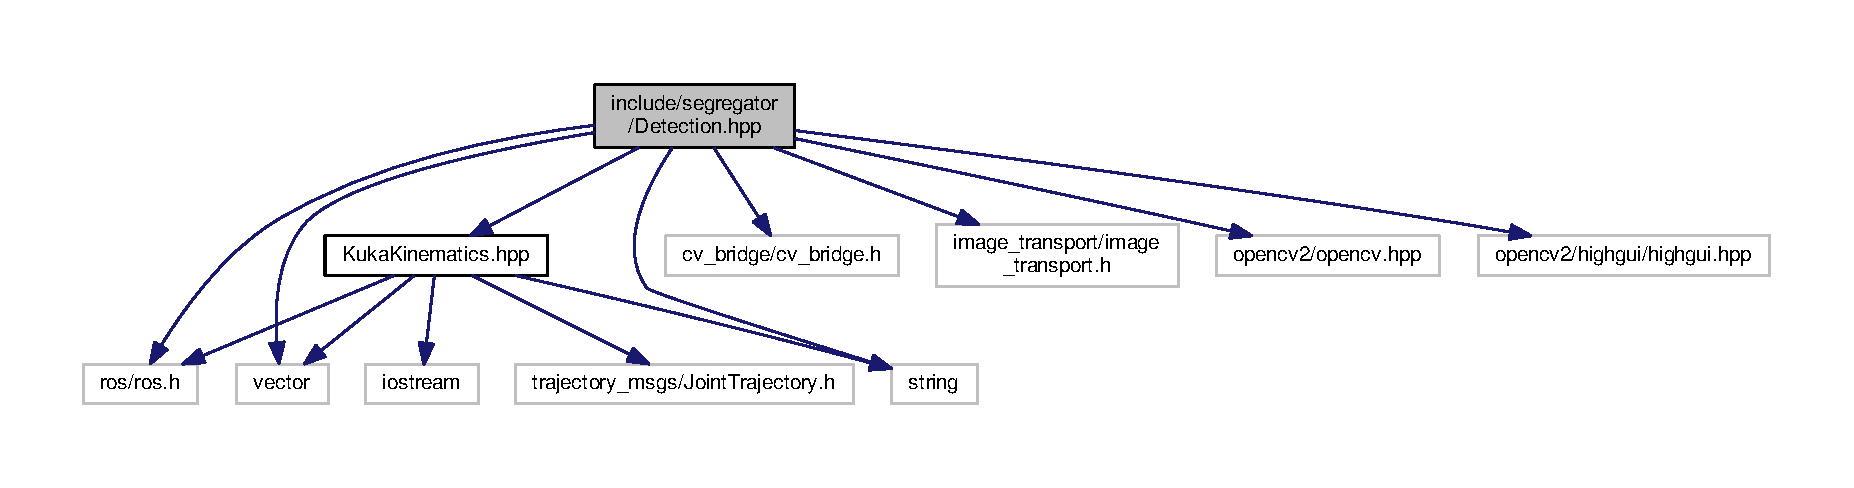
\includegraphics[width=350pt]{Detection_8hpp__incl}
\end{center}
\end{figure}
This graph shows which files directly or indirectly include this file\+:\nopagebreak
\begin{figure}[H]
\begin{center}
\leavevmode
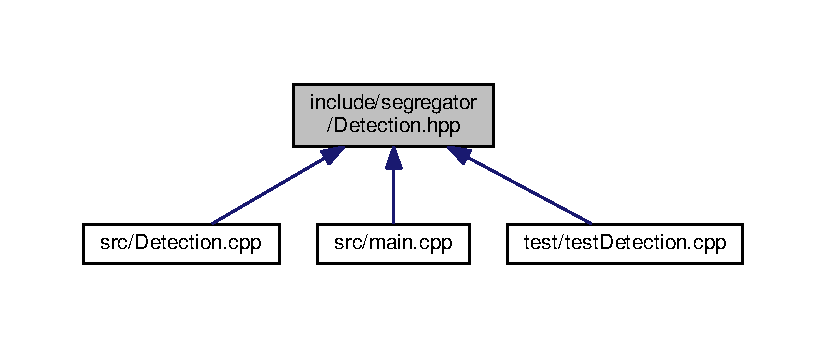
\includegraphics[width=350pt]{Detection_8hpp__dep__incl}
\end{center}
\end{figure}
\subsection*{Classes}
\begin{DoxyCompactItemize}
\item 
class \hyperlink{classDetection}{Detection}
\end{DoxyCompactItemize}

\hypertarget{Gripper_8hpp}{}\section{include/segregator/\+Gripper.hpp File Reference}
\label{Gripper_8hpp}\index{include/segregator/\+Gripper.\+hpp@{include/segregator/\+Gripper.\+hpp}}
{\ttfamily \#include $<$std\+\_\+srvs/\+Empty.\+h$>$}\\*
{\ttfamily \#include $<$std\+\_\+msgs/\+Bool.\+h$>$}\\*
{\ttfamily \#include $<$ros/ros.\+h$>$}\\*
{\ttfamily \#include $<$iostream$>$}\\*
Include dependency graph for Gripper.\+hpp\+:\nopagebreak
\begin{figure}[H]
\begin{center}
\leavevmode
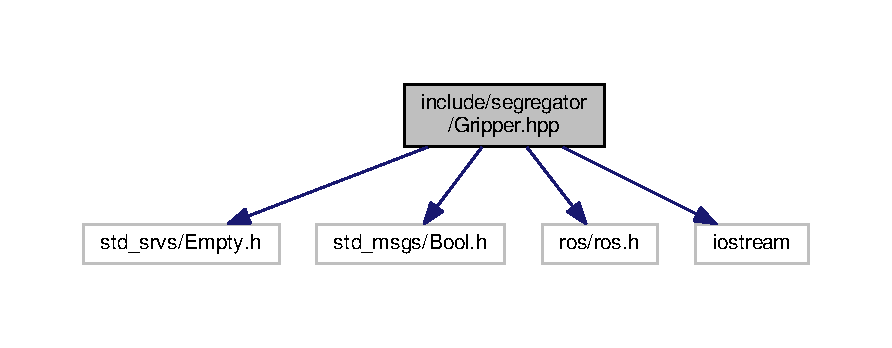
\includegraphics[width=350pt]{Gripper_8hpp__incl}
\end{center}
\end{figure}
This graph shows which files directly or indirectly include this file\+:\nopagebreak
\begin{figure}[H]
\begin{center}
\leavevmode
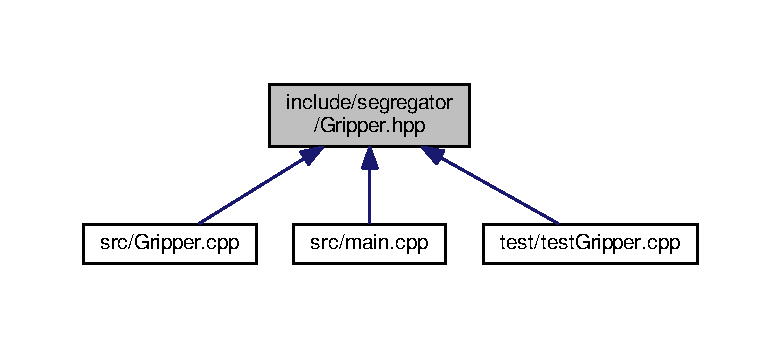
\includegraphics[width=350pt]{Gripper_8hpp__dep__incl}
\end{center}
\end{figure}
\subsection*{Classes}
\begin{DoxyCompactItemize}
\item 
class \hyperlink{classKukaGripper}{Kuka\+Gripper}
\end{DoxyCompactItemize}

\hypertarget{KukaKinematics_8hpp}{}\section{include/segregator/\+Kuka\+Kinematics.hpp File Reference}
\label{KukaKinematics_8hpp}\index{include/segregator/\+Kuka\+Kinematics.\+hpp@{include/segregator/\+Kuka\+Kinematics.\+hpp}}
{\ttfamily \#include $<$ros/ros.\+h$>$}\\*
{\ttfamily \#include $<$trajectory\+\_\+msgs/\+Joint\+Trajectory.\+h$>$}\\*
{\ttfamily \#include $<$iostream$>$}\\*
{\ttfamily \#include $<$vector$>$}\\*
{\ttfamily \#include $<$string$>$}\\*
Include dependency graph for Kuka\+Kinematics.\+hpp\+:\nopagebreak
\begin{figure}[H]
\begin{center}
\leavevmode
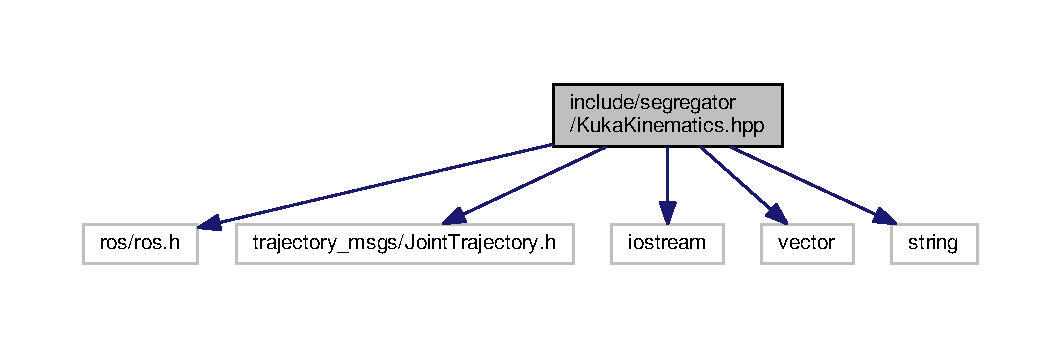
\includegraphics[width=350pt]{KukaKinematics_8hpp__incl}
\end{center}
\end{figure}
This graph shows which files directly or indirectly include this file\+:\nopagebreak
\begin{figure}[H]
\begin{center}
\leavevmode
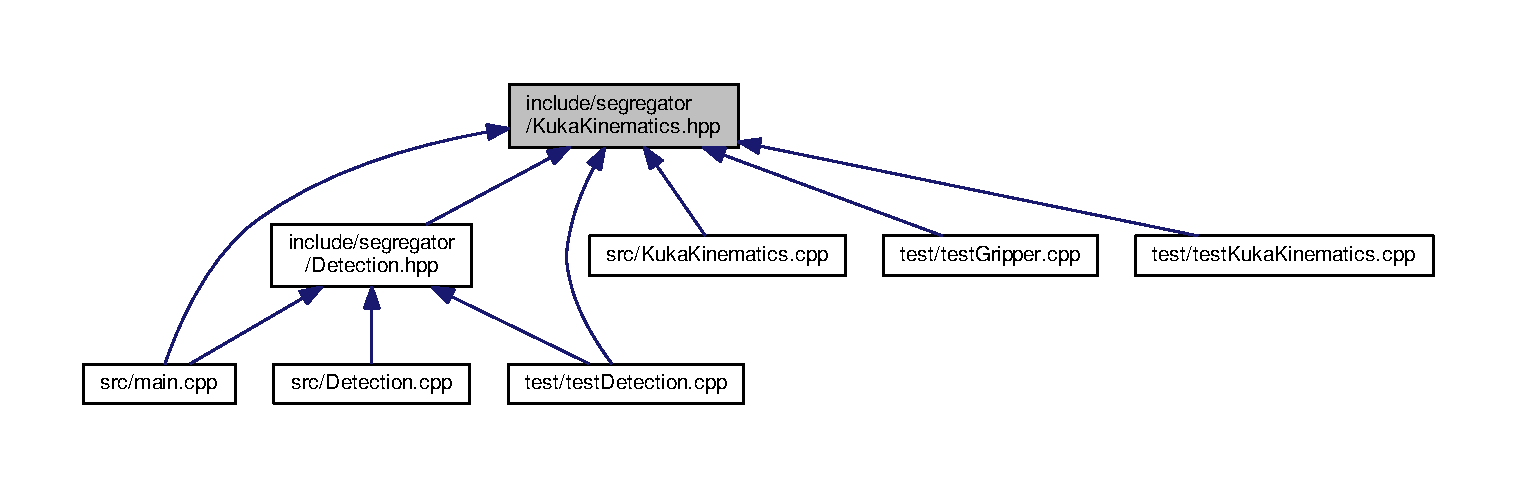
\includegraphics[width=350pt]{KukaKinematics_8hpp__dep__incl}
\end{center}
\end{figure}
\subsection*{Classes}
\begin{DoxyCompactItemize}
\item 
class \hyperlink{classKukaKinematics}{Kuka\+Kinematics}
\end{DoxyCompactItemize}

\hypertarget{README_8md}{}\section{R\+E\+A\+D\+M\+E.\+md File Reference}
\label{README_8md}\index{R\+E\+A\+D\+M\+E.\+md@{R\+E\+A\+D\+M\+E.\+md}}

\hypertarget{cppcheck_8txt}{}\section{results/cppcheck.txt File Reference}
\label{cppcheck_8txt}\index{results/cppcheck.\+txt@{results/cppcheck.\+txt}}

\hypertarget{cpplint_8txt}{}\section{results/cpplint.txt File Reference}
\label{cpplint_8txt}\index{results/cpplint.\+txt@{results/cpplint.\+txt}}
\subsection*{Variables}
\begin{DoxyCompactItemize}
\item 
src \hyperlink{test_2main_8cpp_a3c04138a5bfe5d72780bb7e82a18e627}{main} \hyperlink{cpplint_8txt_a75aa4eb49cbd493e20a62f4d44489c69}{cpp}
\end{DoxyCompactItemize}


\subsection{Variable Documentation}
\index{cpplint.\+txt@{cpplint.\+txt}!cpp@{cpp}}
\index{cpp@{cpp}!cpplint.\+txt@{cpplint.\+txt}}
\subsubsection[{\texorpdfstring{cpp}{cpp}}]{\setlength{\rightskip}{0pt plus 5cm}src {\bf main} cpp}\hypertarget{cpplint_8txt_a75aa4eb49cbd493e20a62f4d44489c69}{}\label{cpplint_8txt_a75aa4eb49cbd493e20a62f4d44489c69}

\hypertarget{Detection_8cpp}{}\section{src/\+Detection.cpp File Reference}
\label{Detection_8cpp}\index{src/\+Detection.\+cpp@{src/\+Detection.\+cpp}}
{\ttfamily \#include \char`\"{}Detection.\+hpp\char`\"{}}\\*
{\ttfamily \#include $<$opencv2/core/core.\+hpp$>$}\\*
{\ttfamily \#include $<$opencv2/highgui/highgui.\+hpp$>$}\\*
Include dependency graph for Detection.\+cpp\+:\nopagebreak
\begin{figure}[H]
\begin{center}
\leavevmode
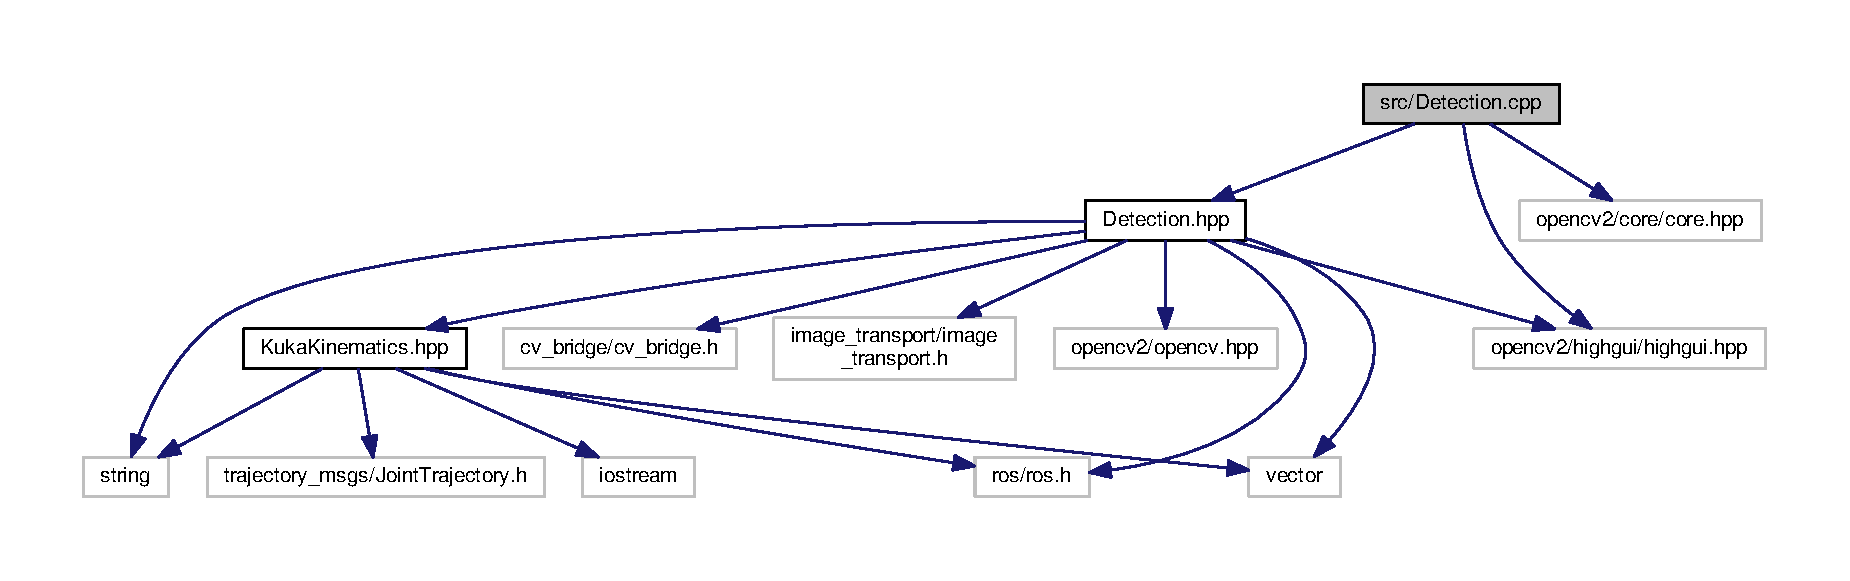
\includegraphics[width=350pt]{Detection_8cpp__incl}
\end{center}
\end{figure}

\hypertarget{Gripper_8cpp}{}\section{src/\+Gripper.cpp File Reference}
\label{Gripper_8cpp}\index{src/\+Gripper.\+cpp@{src/\+Gripper.\+cpp}}
{\ttfamily \#include \char`\"{}Gripper.\+hpp\char`\"{}}\\*
Include dependency graph for Gripper.\+cpp\+:\nopagebreak
\begin{figure}[H]
\begin{center}
\leavevmode
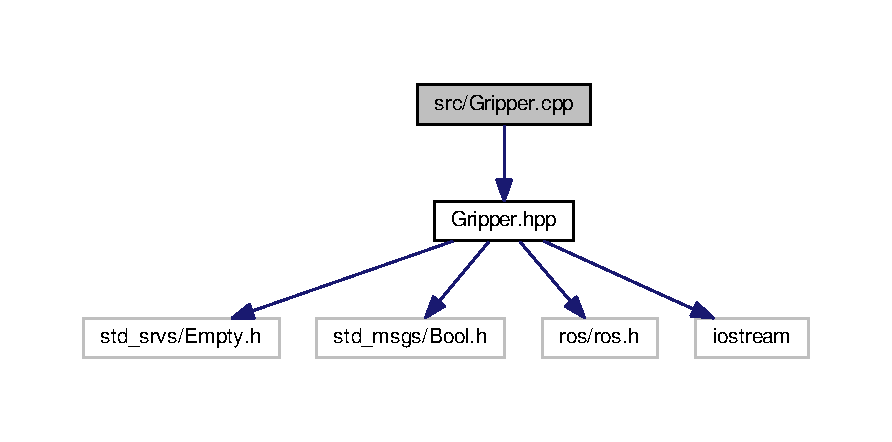
\includegraphics[width=350pt]{Gripper_8cpp__incl}
\end{center}
\end{figure}

\hypertarget{KukaKinematics_8cpp}{}\section{src/\+Kuka\+Kinematics.cpp File Reference}
\label{KukaKinematics_8cpp}\index{src/\+Kuka\+Kinematics.\+cpp@{src/\+Kuka\+Kinematics.\+cpp}}
{\ttfamily \#include \char`\"{}Kuka\+Kinematics.\+hpp\char`\"{}}\\*
Include dependency graph for Kuka\+Kinematics.\+cpp\+:\nopagebreak
\begin{figure}[H]
\begin{center}
\leavevmode
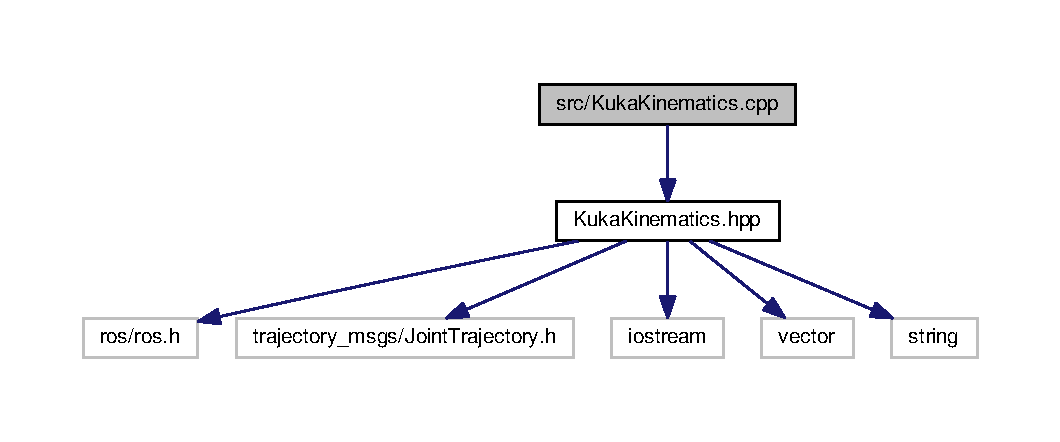
\includegraphics[width=350pt]{KukaKinematics_8cpp__incl}
\end{center}
\end{figure}

\hypertarget{src_2main_8cpp}{}\section{src/main.cpp File Reference}
\label{src_2main_8cpp}\index{src/main.\+cpp@{src/main.\+cpp}}
{\ttfamily \#include $<$iostream$>$}\\*
{\ttfamily \#include \char`\"{}Kuka\+Kinematics.\+hpp\char`\"{}}\\*
{\ttfamily \#include \char`\"{}Gripper.\+hpp\char`\"{}}\\*
{\ttfamily \#include \char`\"{}Detection.\+hpp\char`\"{}}\\*
{\ttfamily \#include \char`\"{}sensor\+\_\+msgs/\+Image.\+h\char`\"{}}\\*
Include dependency graph for main.\+cpp\+:\nopagebreak
\begin{figure}[H]
\begin{center}
\leavevmode
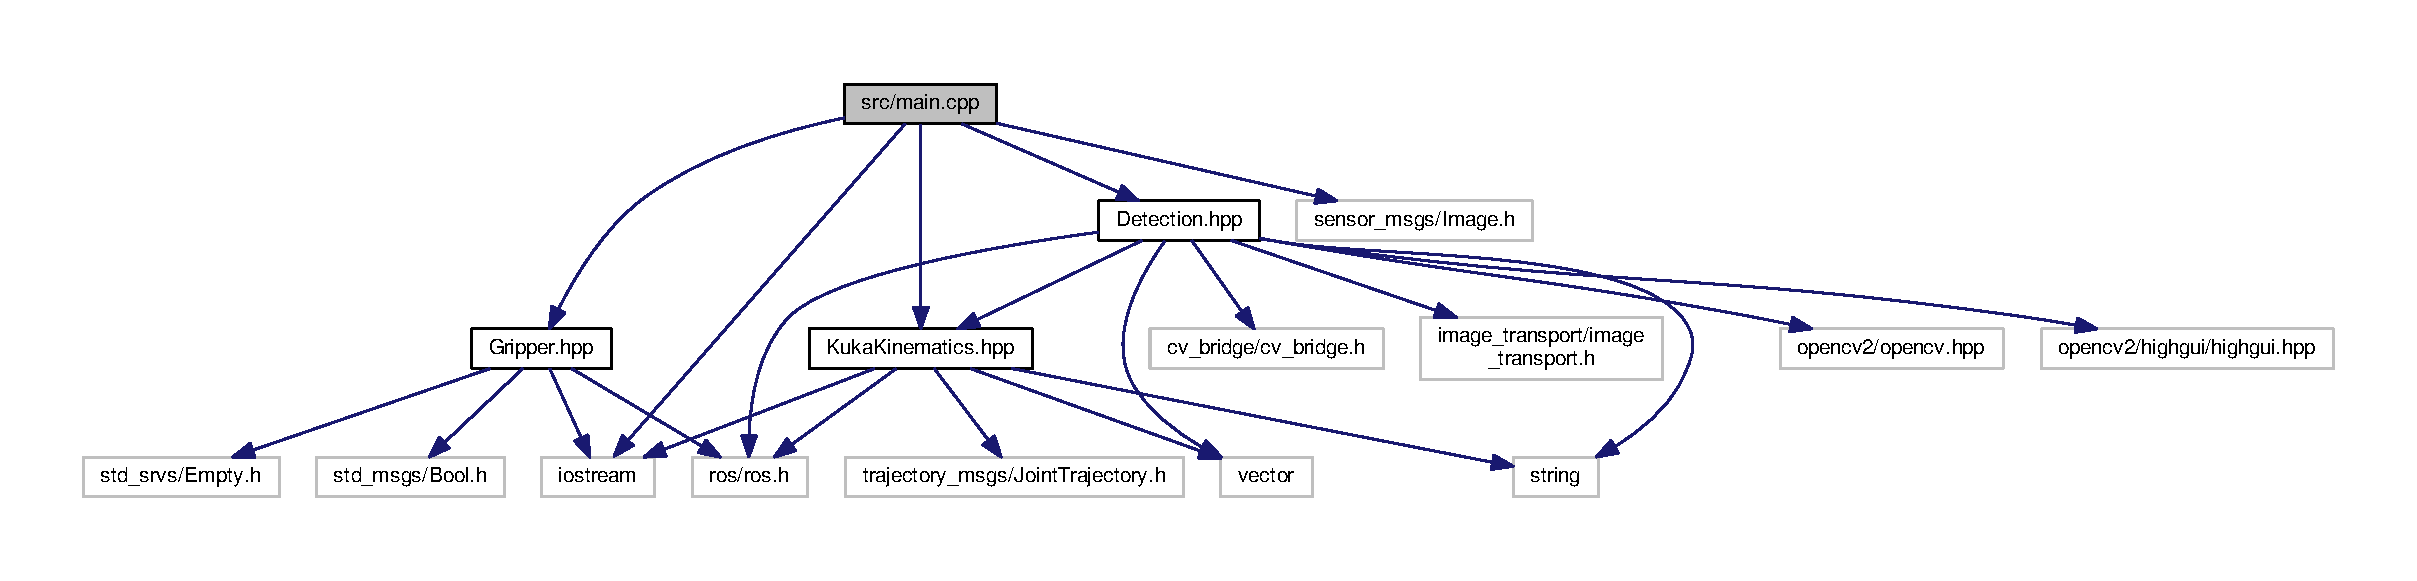
\includegraphics[width=350pt]{src_2main_8cpp__incl}
\end{center}
\end{figure}
\subsection*{Functions}
\begin{DoxyCompactItemize}
\item 
void \hyperlink{src_2main_8cpp_a67096dd66789a3dd47695d0504564549}{image\+Cb} (const sensor\+\_\+msgs\+::\+Image\+Const\+Ptr \&msg)
\item 
int \hyperlink{src_2main_8cpp_a3c04138a5bfe5d72780bb7e82a18e627}{main} (int argc, char $\ast$$\ast$argv)
\end{DoxyCompactItemize}
\subsection*{Variables}
\begin{DoxyCompactItemize}
\item 
int \hyperlink{src_2main_8cpp_adf916204820072417ed73a32de1cefcf}{flag} = 0
\end{DoxyCompactItemize}


\subsection{Function Documentation}
\index{src/main.\+cpp@{src/main.\+cpp}!image\+Cb@{image\+Cb}}
\index{image\+Cb@{image\+Cb}!src/main.\+cpp@{src/main.\+cpp}}
\subsubsection[{\texorpdfstring{image\+Cb(const sensor\+\_\+msgs\+::\+Image\+Const\+Ptr \&msg)}{imageCb(const sensor_msgs::ImageConstPtr &msg)}}]{\setlength{\rightskip}{0pt plus 5cm}void image\+Cb (
\begin{DoxyParamCaption}
\item[{const sensor\+\_\+msgs\+::\+Image\+Const\+Ptr \&}]{msg}
\end{DoxyParamCaption}
)}\hypertarget{src_2main_8cpp_a67096dd66789a3dd47695d0504564549}{}\label{src_2main_8cpp_a67096dd66789a3dd47695d0504564549}
\index{src/main.\+cpp@{src/main.\+cpp}!main@{main}}
\index{main@{main}!src/main.\+cpp@{src/main.\+cpp}}
\subsubsection[{\texorpdfstring{main(int argc, char $\ast$$\ast$argv)}{main(int argc, char **argv)}}]{\setlength{\rightskip}{0pt plus 5cm}int main (
\begin{DoxyParamCaption}
\item[{int}]{argc, }
\item[{char $\ast$$\ast$}]{argv}
\end{DoxyParamCaption}
)}\hypertarget{src_2main_8cpp_a3c04138a5bfe5d72780bb7e82a18e627}{}\label{src_2main_8cpp_a3c04138a5bfe5d72780bb7e82a18e627}


\subsection{Variable Documentation}
\index{src/main.\+cpp@{src/main.\+cpp}!flag@{flag}}
\index{flag@{flag}!src/main.\+cpp@{src/main.\+cpp}}
\subsubsection[{\texorpdfstring{flag}{flag}}]{\setlength{\rightskip}{0pt plus 5cm}int flag = 0}\hypertarget{src_2main_8cpp_adf916204820072417ed73a32de1cefcf}{}\label{src_2main_8cpp_adf916204820072417ed73a32de1cefcf}

\hypertarget{test_2main_8cpp}{}\section{test/main.cpp File Reference}
\label{test_2main_8cpp}\index{test/main.\+cpp@{test/main.\+cpp}}
{\ttfamily \#include $<$gtest/gtest.\+h$>$}\\*
{\ttfamily \#include $<$ros/ros.\+h$>$}\\*
Include dependency graph for main.\+cpp\+:\nopagebreak
\begin{figure}[H]
\begin{center}
\leavevmode
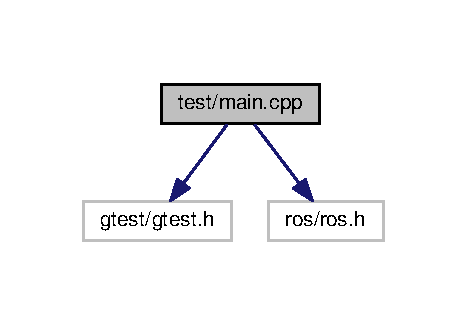
\includegraphics[width=224pt]{test_2main_8cpp__incl}
\end{center}
\end{figure}
\subsection*{Functions}
\begin{DoxyCompactItemize}
\item 
int \hyperlink{test_2main_8cpp_a3c04138a5bfe5d72780bb7e82a18e627}{main} (int argc, char $\ast$$\ast$argv)
\end{DoxyCompactItemize}


\subsection{Function Documentation}
\index{test/main.\+cpp@{test/main.\+cpp}!main@{main}}
\index{main@{main}!test/main.\+cpp@{test/main.\+cpp}}
\subsubsection[{\texorpdfstring{main(int argc, char $\ast$$\ast$argv)}{main(int argc, char **argv)}}]{\setlength{\rightskip}{0pt plus 5cm}int main (
\begin{DoxyParamCaption}
\item[{int}]{argc, }
\item[{char $\ast$$\ast$}]{argv}
\end{DoxyParamCaption}
)}\hypertarget{test_2main_8cpp_a3c04138a5bfe5d72780bb7e82a18e627}{}\label{test_2main_8cpp_a3c04138a5bfe5d72780bb7e82a18e627}

\hypertarget{testDetection_8cpp}{}\section{test/test\+Detection.cpp File Reference}
\label{testDetection_8cpp}\index{test/test\+Detection.\+cpp@{test/test\+Detection.\+cpp}}
{\ttfamily \#include $<$gtest/gtest.\+h$>$}\\*
{\ttfamily \#include \char`\"{}Kuka\+Kinematics.\+hpp\char`\"{}}\\*
{\ttfamily \#include \char`\"{}Detection.\+hpp\char`\"{}}\\*
Include dependency graph for test\+Detection.\+cpp\+:\nopagebreak
\begin{figure}[H]
\begin{center}
\leavevmode
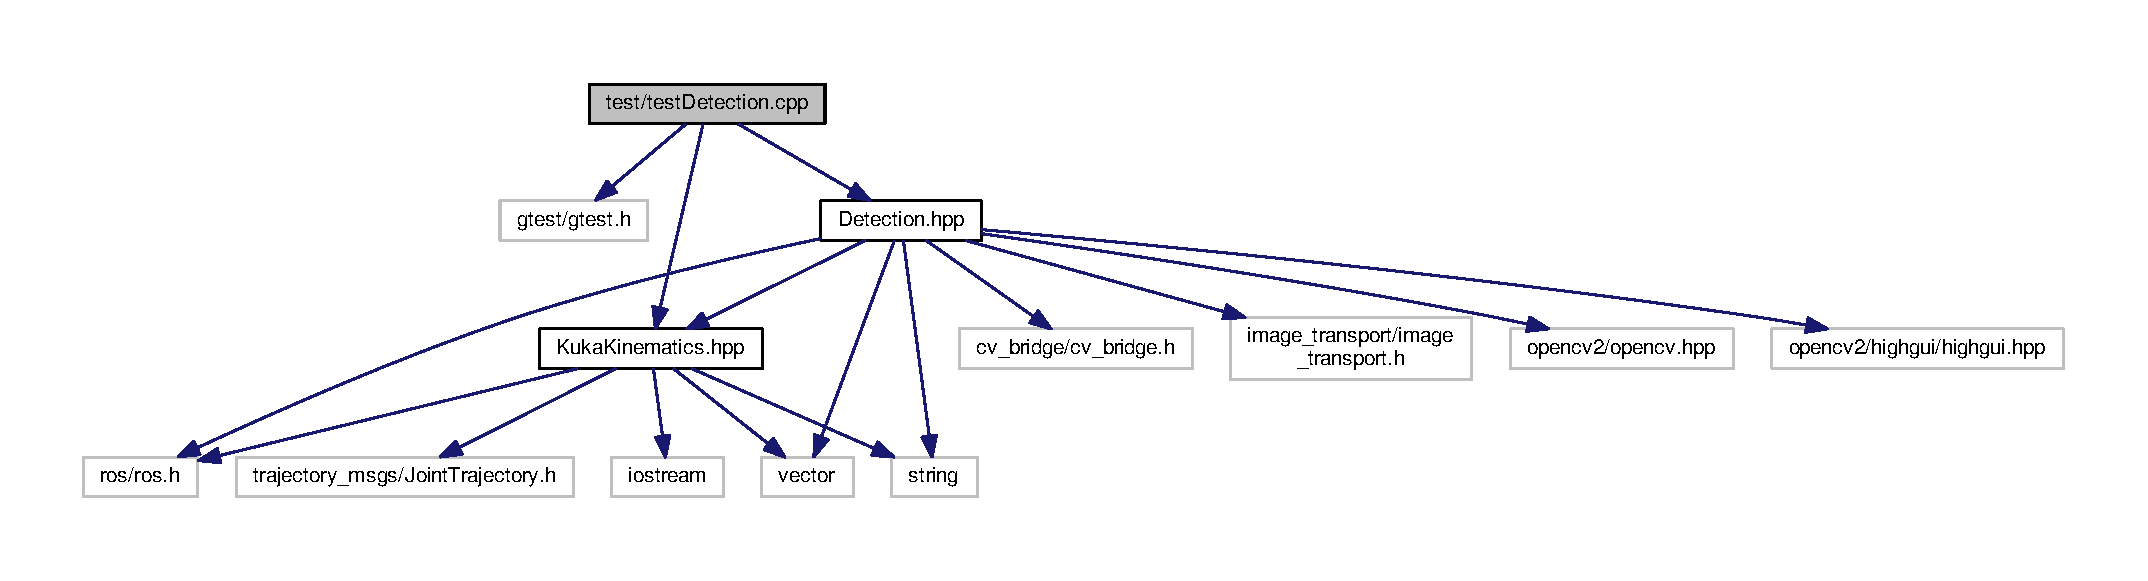
\includegraphics[width=350pt]{testDetection_8cpp__incl}
\end{center}
\end{figure}
\subsection*{Functions}
\begin{DoxyCompactItemize}
\item 
\hyperlink{testDetection_8cpp_a13db54a77daeda02927f6c9f65217219}{T\+E\+ST} (Detection\+Test, test\+Color\+Thresholder)
\begin{DoxyCompactList}\small\item\em This is the google test for the first method of the class. \end{DoxyCompactList}\end{DoxyCompactItemize}


\subsection{Function Documentation}
\index{test\+Detection.\+cpp@{test\+Detection.\+cpp}!T\+E\+ST@{T\+E\+ST}}
\index{T\+E\+ST@{T\+E\+ST}!test\+Detection.\+cpp@{test\+Detection.\+cpp}}
\subsubsection[{\texorpdfstring{T\+E\+S\+T(\+Detection\+Test, test\+Color\+Thresholder)}{TEST(DetectionTest, testColorThresholder)}}]{\setlength{\rightskip}{0pt plus 5cm}T\+E\+ST (
\begin{DoxyParamCaption}
\item[{Detection\+Test}]{, }
\item[{test\+Color\+Thresholder}]{}
\end{DoxyParamCaption}
)}\hypertarget{testDetection_8cpp_a13db54a77daeda02927f6c9f65217219}{}\label{testDetection_8cpp_a13db54a77daeda02927f6c9f65217219}


This is the google test for the first method of the class. 


\hypertarget{testGripper_8cpp}{}\section{test/test\+Gripper.cpp File Reference}
\label{testGripper_8cpp}\index{test/test\+Gripper.\+cpp@{test/test\+Gripper.\+cpp}}
{\ttfamily \#include $<$gtest/gtest.\+h$>$}\\*
{\ttfamily \#include \char`\"{}Kuka\+Kinematics.\+hpp\char`\"{}}\\*
{\ttfamily \#include \char`\"{}Gripper.\+hpp\char`\"{}}\\*
Include dependency graph for test\+Gripper.\+cpp\+:\nopagebreak
\begin{figure}[H]
\begin{center}
\leavevmode
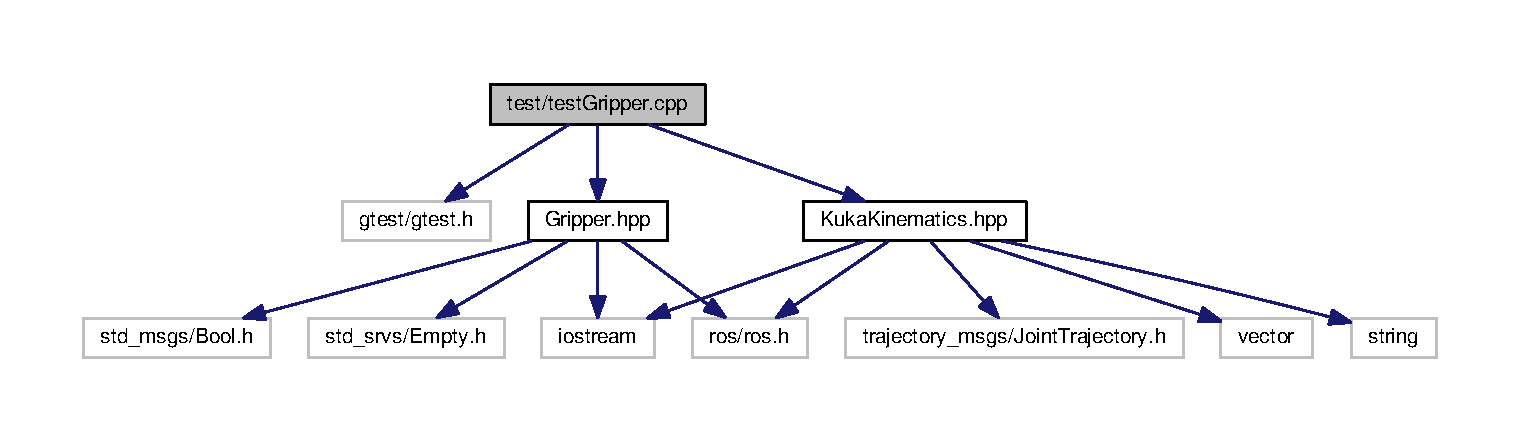
\includegraphics[width=350pt]{testGripper_8cpp__incl}
\end{center}
\end{figure}
\subsection*{Functions}
\begin{DoxyCompactItemize}
\item 
\hyperlink{testGripper_8cpp_a0513323fd8e2daccfc3f517b385cccda}{T\+E\+ST} (Kuka\+Gripper\+Test, test\+Get\+Gripper\+State)
\begin{DoxyCompactList}\small\item\em This is the google test for the second method of the class. \end{DoxyCompactList}\item 
\hyperlink{testGripper_8cpp_a27540b6d36cbda55cbbfc4c86cc2980e}{T\+E\+ST} (Kuka\+Gripper\+Test, test\+Gripper\+Toggle)
\begin{DoxyCompactList}\small\item\em This is the google test for the first method of the class. \end{DoxyCompactList}\end{DoxyCompactItemize}


\subsection{Function Documentation}
\index{test\+Gripper.\+cpp@{test\+Gripper.\+cpp}!T\+E\+ST@{T\+E\+ST}}
\index{T\+E\+ST@{T\+E\+ST}!test\+Gripper.\+cpp@{test\+Gripper.\+cpp}}
\subsubsection[{\texorpdfstring{T\+E\+S\+T(\+Kuka\+Gripper\+Test, test\+Get\+Gripper\+State)}{TEST(KukaGripperTest, testGetGripperState)}}]{\setlength{\rightskip}{0pt plus 5cm}T\+E\+ST (
\begin{DoxyParamCaption}
\item[{Kuka\+Gripper\+Test}]{, }
\item[{test\+Get\+Gripper\+State}]{}
\end{DoxyParamCaption}
)}\hypertarget{testGripper_8cpp_a0513323fd8e2daccfc3f517b385cccda}{}\label{testGripper_8cpp_a0513323fd8e2daccfc3f517b385cccda}


This is the google test for the second method of the class. 

\index{test\+Gripper.\+cpp@{test\+Gripper.\+cpp}!T\+E\+ST@{T\+E\+ST}}
\index{T\+E\+ST@{T\+E\+ST}!test\+Gripper.\+cpp@{test\+Gripper.\+cpp}}
\subsubsection[{\texorpdfstring{T\+E\+S\+T(\+Kuka\+Gripper\+Test, test\+Gripper\+Toggle)}{TEST(KukaGripperTest, testGripperToggle)}}]{\setlength{\rightskip}{0pt plus 5cm}T\+E\+ST (
\begin{DoxyParamCaption}
\item[{Kuka\+Gripper\+Test}]{, }
\item[{test\+Gripper\+Toggle}]{}
\end{DoxyParamCaption}
)}\hypertarget{testGripper_8cpp_a27540b6d36cbda55cbbfc4c86cc2980e}{}\label{testGripper_8cpp_a27540b6d36cbda55cbbfc4c86cc2980e}


This is the google test for the first method of the class. 


\hypertarget{testKukaKinematics_8cpp}{}\section{test/test\+Kuka\+Kinematics.cpp File Reference}
\label{testKukaKinematics_8cpp}\index{test/test\+Kuka\+Kinematics.\+cpp@{test/test\+Kuka\+Kinematics.\+cpp}}
{\ttfamily \#include $<$gtest/gtest.\+h$>$}\\*
{\ttfamily \#include \char`\"{}Kuka\+Kinematics.\+hpp\char`\"{}}\\*
Include dependency graph for test\+Kuka\+Kinematics.\+cpp\+:\nopagebreak
\begin{figure}[H]
\begin{center}
\leavevmode
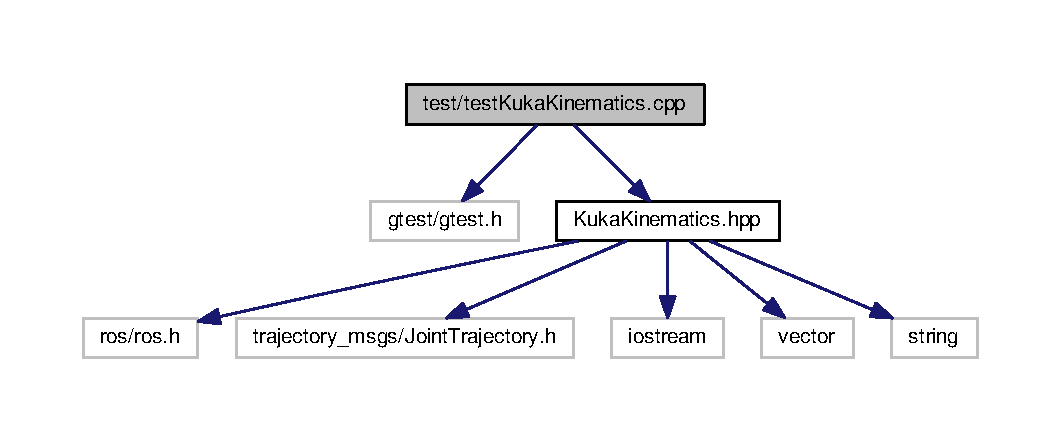
\includegraphics[width=350pt]{testKukaKinematics_8cpp__incl}
\end{center}
\end{figure}
\subsection*{Functions}
\begin{DoxyCompactItemize}
\item 
void \hyperlink{testKukaKinematics_8cpp_a2a150d121c051ba60c471c6f61249119}{callback} (const trajectory\+\_\+msgs\+::\+Joint\+Trajectory \&pub\+Command)
\item 
\hyperlink{testKukaKinematics_8cpp_afb70f40ac51d06a3427c46223bf7d285}{T\+E\+ST} (Kuka\+Kinematics\+Test, test\+Send\+Robot\+To\+Pos)
\end{DoxyCompactItemize}
\subsection*{Variables}
\begin{DoxyCompactItemize}
\item 
trajectory\+\_\+msgs\+::\+Joint\+Trajectory \hyperlink{testKukaKinematics_8cpp_a2a85af2f0424d03cf0dc6410e4cfebd1}{command}
\end{DoxyCompactItemize}


\subsection{Function Documentation}
\index{test\+Kuka\+Kinematics.\+cpp@{test\+Kuka\+Kinematics.\+cpp}!callback@{callback}}
\index{callback@{callback}!test\+Kuka\+Kinematics.\+cpp@{test\+Kuka\+Kinematics.\+cpp}}
\subsubsection[{\texorpdfstring{callback(const trajectory\+\_\+msgs\+::\+Joint\+Trajectory \&pub\+Command)}{callback(const trajectory_msgs::JointTrajectory &pubCommand)}}]{\setlength{\rightskip}{0pt plus 5cm}void callback (
\begin{DoxyParamCaption}
\item[{const trajectory\+\_\+msgs\+::\+Joint\+Trajectory \&}]{pub\+Command}
\end{DoxyParamCaption}
)}\hypertarget{testKukaKinematics_8cpp_a2a150d121c051ba60c471c6f61249119}{}\label{testKukaKinematics_8cpp_a2a150d121c051ba60c471c6f61249119}
\index{test\+Kuka\+Kinematics.\+cpp@{test\+Kuka\+Kinematics.\+cpp}!T\+E\+ST@{T\+E\+ST}}
\index{T\+E\+ST@{T\+E\+ST}!test\+Kuka\+Kinematics.\+cpp@{test\+Kuka\+Kinematics.\+cpp}}
\subsubsection[{\texorpdfstring{T\+E\+S\+T(\+Kuka\+Kinematics\+Test, test\+Send\+Robot\+To\+Pos)}{TEST(KukaKinematicsTest, testSendRobotToPos)}}]{\setlength{\rightskip}{0pt plus 5cm}T\+E\+ST (
\begin{DoxyParamCaption}
\item[{Kuka\+Kinematics\+Test}]{, }
\item[{test\+Send\+Robot\+To\+Pos}]{}
\end{DoxyParamCaption}
)}\hypertarget{testKukaKinematics_8cpp_afb70f40ac51d06a3427c46223bf7d285}{}\label{testKukaKinematics_8cpp_afb70f40ac51d06a3427c46223bf7d285}


\subsection{Variable Documentation}
\index{test\+Kuka\+Kinematics.\+cpp@{test\+Kuka\+Kinematics.\+cpp}!command@{command}}
\index{command@{command}!test\+Kuka\+Kinematics.\+cpp@{test\+Kuka\+Kinematics.\+cpp}}
\subsubsection[{\texorpdfstring{command}{command}}]{\setlength{\rightskip}{0pt plus 5cm}trajectory\+\_\+msgs\+::\+Joint\+Trajectory command}\hypertarget{testKukaKinematics_8cpp_a2a85af2f0424d03cf0dc6410e4cfebd1}{}\label{testKukaKinematics_8cpp_a2a85af2f0424d03cf0dc6410e4cfebd1}

%--- End generated contents ---

% Index
\backmatter
\newpage
\phantomsection
\clearemptydoublepage
\addcontentsline{toc}{chapter}{Index}
\printindex

\end{document}
